\chapter{RESULTADOS PRELIMINARES E ESPERADOS}
\label{cap:resultados}

\section{Resultados Preliminares}

Uma etapa determinante no desenvolvimento do sistema de identificação de condutores é a comprovação de viabilidade do mesmo. Para tal foram executados experimentos com classificadores \textit{batch} em conjunto com métodos de processamento de dados. O objetivo dos testes é de se obter um valor alto de precisão (acertos entre condutores autorizados e não autorizados). A configuração destes experimentos está explanada no Capítulo~\ref{cap:metodologia} do presente projeto de pesquisa. Os gráficos da Figura~\ref{fig:janelas} mostram o desempenho em termos da acurácia dos testes com a dispersão dos resultados dos classificadores, divididos em cada umas das técnicas de redução de dimensionalidade.

Em todos os cenários, o classificador KNN obteve desempenho superior em comparação aos outros classificadores, enquanto o RNA teve um desempenho consideravelmente inferior, além de apresentar valores de desvio padrão superiores, se mostrando uma técnica pouco indicada para a tarefa de identificação de condutores.

Considerando a janela temporal ideal para a identificação de condutores, conclui-se que a janela de 90 segundos maximiza o desempenho do classificador KNN, porém, nos casos das técnicas RNA e RF, quanto maior a janela temporal, melhor a taxa de acertos dos mesmos. A janela temporal de 30 segundos apresentou desempenho inferior no KNN e RF, enquanto no caso do RNA, os valores se estabilizaram a partir da janela de 30 segundo, com acréscimo razoável na janela de 120 segundos. 

Pode-se observar que a janela de 90 segundos tem o melhor desempenho no que diz respeito aos certos quanto à autenticidade do condutor. É valido ressaltar que, em aplicações reais futuras, deve-se determinar um valor de janela ótimo que alie a rapidez e precisão na identificação do condutor, visto que uma janela de 90 segundo pode ser muito quanto se trata de uma ação criminosa, porém, um falso negativo é uma situação que deve ser evitada para a confiabilidade do sistema.

\begin{figure}[!ht]
	\centering
	\subfloat[\label{fig:janPCA}][PCA]{%
		\includegraphics[width=0.55\textwidth]{PCA.eps}
	}
%	\hfill
	\subfloat[\label{fig:janIPCA}][IPCA]{%
		\includegraphics[width=0.55\textwidth]{IPCA.eps}
	}\\
	\subfloat[\label{fig:janICA}][ICA]{%
		\includegraphics[width=0.55\textwidth]{ICA.eps}
	}
	\caption{Precisão média de cada método de redução de dimensionalidade.}
	\label{fig:janelas}
	{\small Fonte: Próprio autor.} %Fonte da imagem
\end{figure}


Com relação à eficiência dos métodos de redução de dimensionalidade, nenhumas das técnicas se mostrou superior em questão de desempenho em comparação às outras, no qual o objetivo de diminuir o espaço amostral de entrada do classificador foi alcançado sem que se houvesse comprometimento na classificação.

No caso do melhor classificador, o KNN, as três técnicas obtiveram uma quantidade de acertos semelhantes nas mesmas condições de janela temporal. Contudo, nos classificadores RF e RNA não houve uma técnica que teve seu desempenho superior em todas as circunstâncias. Os gráficos apresentados na Figura~\ref{fig:reducao} ilustram o desempenho comparado de cada uma das técnicas de redução de dimensionalidade em cada um dos classificadores abordados.

\begin{figure}[!ht]
	\centering
	\subfloat[\label{fig:KNN}][KNN]{%
		\includegraphics[width=0.55\textwidth]{KNN.eps}
	}
	%	\hfill
	\subfloat[\label{fig:RF}][RF]{%
		\includegraphics[width=0.55\textwidth]{RF.eps}
	}

	\subfloat[\label{fig:RNA}][RNA]{%
		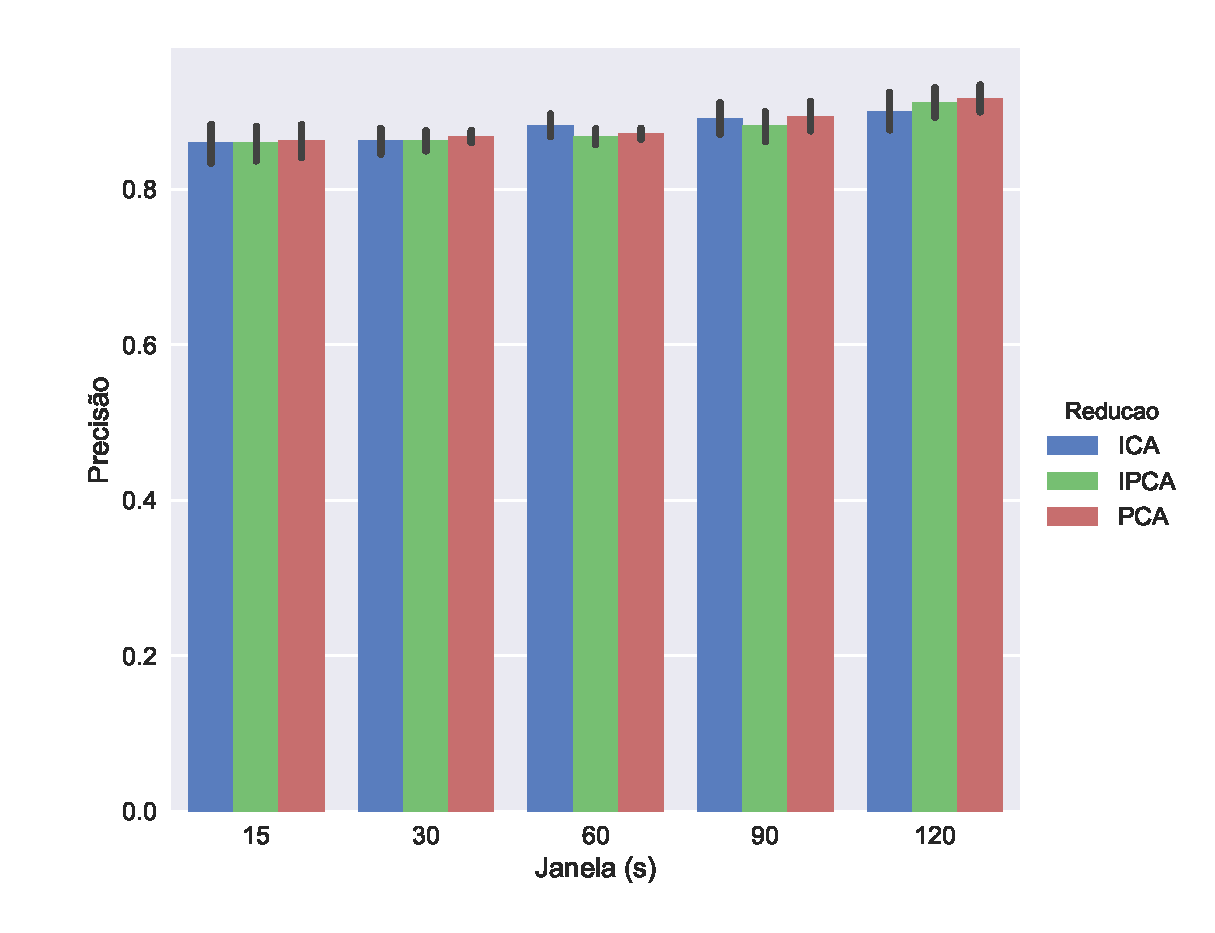
\includegraphics[width=0.55\textwidth]{MLP.eps}
	}
	\caption{Precisão média de cada classificador por método de redução de dimensionalidade.}
	\label{fig:reducao}
	{\small Fonte: Próprio autor.} %Fonte da imagem
\end{figure}

A Tabelas~\ref{tab:desKNN}, \ref{tab:desRF} e \ref{tab:desRNA} apresentam uma análise de desempenho mais aprofundada dos classificadores, considerando, além da precisão, as métricas de análise de concordância \textit{Cohen's kappa Score} e \textit{F1-Score}. Para o classificador kNN o valor do desvio padrão foi insignificante e, portanto, foi desconsiderado. No caso do classificador kNN, pode-se observar que em todos os casos, a janela de 90 segundos resulta em um resultado melhor chegando à 99.5\% de acertos com redução PCA e ICA e 99.4\% na redução IPCA. Por sua vez, o classificador \textit{Random Forest} A janela de 120 segundos foi a que obteve o melhor desempenho, chegando precisão média chegando à 95.2\%, com concordância de 88.4\%, mostrando que quanto mais tempo usado no janelamento, melhor o seu desempenho, o que pode ser um ponto negativo, devido ao tempo excessivo para o início da identificação dos condutores. Já a RNA teve um desempenho inferior aos demais chegando na precisão máxima de 88.1\% com apenas de 71.3\% de concordância (considerando o desequilíbrio das classes).

\begin{table}[!htb]
	\centering
	\caption{Desempenho do Classificador KNN e Técnicas de Redução de Dimensionalidade em diferentes métricas}
	\label{tab:desKNN}
	\resizebox{1\textwidth}{!}{
	\begin{tabular}{cccccccccc}
		\hline
		\multicolumn{10}{c}{kNN} \\ \hline
		\multirow{2}{*}{Janela (s)} & \multicolumn{3}{c}{PCA} & \multicolumn{3}{c}{IPCA} & \multicolumn{3}{c}{ICA} \\ \cline{2-10} 
		&  Precisão & F1-Score & Cohen Kappa & \multicolumn{1}{l}{ Precisão} & \multicolumn{1}{l}{F1-Score} & \multicolumn{1}{l}{Cohen Kappa} & \multicolumn{1}{l}{ Precisão} & \multicolumn{1}{l}{F1-Score} & \multicolumn{1}{l}{Cohen Kappa} \\ \hline
		15 & 0.956 & 0.927 & 0.896 & 0.956 & 0.927 & 0.896 & 0.957 & 0.927 & 0.896 \\
		30 & 0.919 & 0.838 & 0.785 & 0.922 & 0.842 & 0.791 & 0.917 & 0.834 & 0.778 \\
		60 & 0.971 & 0.951 & 0.930 & 0.972 & 0.952 & 0.932 & 0.976 & 0.960 & 0.943 \\
		90 & 0.995 & 0.992 & 0.988 & 0.994 & 0.990 & 0.986 & 0.995 & 0.991 & 0.988 \\
		120 & 0.989 & 0.981 & 0.974 & 0.989 & 0.981 & 0.974 & 0.988 & 0.980 & 0.971 \\ \hline
\end{tabular}}
\end{table}


\begin{table}[!htb]
	\centering
	\caption{Desempenho do Classificador \textit{Random Forest} e Técnicas de Redução de Dimensionalidade em diferentes métricas}
	\label{tab:desRF}
	\resizebox{1.\textwidth}{!}{
		\begin{tabular}{cccccccccc}
			\hline
			\multicolumn{10}{c}{Random Forest} \\ \hline
			\multirow{2}{*}{Janela (s)} & \multicolumn{3}{c}{PCA} & \multicolumn{3}{c}{IPCA} & \multicolumn{3}{c}{ICA} \\ \cline{2-10} 
			&  Precisão & F1-Score & Cohen Kappa &  Precisão & F1-Score & Cohen Kappa &  Precisão & F1-Score & Cohen Kappa \\ \hline
			15 & 0.907$\pm$0.001 & 0.841$\pm$0.001 & 0.775$\pm$0.002 & 0.906$\pm$0 & 0.839$\pm$0.001 & 0.773$\pm$0.001 & 0.913$\pm$0.001 & 0.850$\pm$0.002 & 0.791$\pm$0.003 \\
			30 & 0.884$\pm$0 & 0.730$\pm$0.001 & 0.659$\pm$0.001 & 0.887$\pm$0 & 0.737$\pm$0.002 & 0.668$\pm$0.002 & 0.896$\pm$0 & 0.765$\pm$0.001 & 0.701$\pm$0.002 \\
			60 & 0.889$\pm$0.002 & 0.789$\pm$0.005 & 0.712$\pm$0.006 & 0.887$\pm$0.003 & 0.789$\pm$0.005 & 0.713$\pm$0.007 & 0.913$\pm$0.001 & 0.846$\pm$0.002 & 0.786$\pm$0.002 \\
			90 & 0.933$\pm$0.001 & 0.870$\pm$0.002 & 0.825$\pm$0.003 & 0.921$\pm$0.002 & 0.844$\pm$0.004 & 0.792$\pm$0.005 & 0.934$\pm$0.002 & 0.872$\pm$0.004 & 0.828$\pm$0.004 \\
			120 & 0.951$\pm$0.001 & 0.915$\pm$0.002 & 0.881$\pm$0.003 & 0.951$\pm$0.001 & 0.915$\pm$0.002 & 0.880$\pm$0.003 & 0.952$\pm$0.001 & 0.918$\pm$0.002 & 0.884$\pm$0.002 \\ \hline
	\end{tabular}}
\end{table}


\begin{table}[!htb]
	\centering
	\caption{Desempenho do Classificador RNA e Técnicas de Redução de Dimensionalidade em diferentes métricas}
	\label{tab:desRNA}
	\resizebox{1.\textwidth}{!}{
		\begin{tabular}{cccccccccc}
			\hline
			\multicolumn{10}{c}{RNA} \\ \hline
			\multirow{2}{*}{Janela (s)} & \multicolumn{3}{c}{PCA} & \multicolumn{3}{c}{IPCA} & \multicolumn{3}{c}{ICA} \\ \cline{2-10} 
			&  Precisão & F1-Score & Cohen Kappa &  Precisão & F1-Score & Cohen Kappa &  Precisão & F1-Score & Cohen Kappa \\ \hline
			15 & 0.816$\pm$0.021 & 0.678$\pm$0.044 & 0.550$\pm$0.057 & 0.8134$\pm$0.028 & 0.661$\pm$0.078 & 0.535$\pm$0.090 & 0.805$\pm$0.026 & 0.642$\pm$0.065 & 0.510$\pm$0.079 \\
			30 & 0.852$\pm$0.011 & 0.630$\pm$0.045 & 0.546$\pm$0.046 & 0.838$\pm$0.026 & 0.592$\pm$0.088 & 0.501$\pm$0.096 & 0.828$\pm$0.23 & 0.538$\pm$0.091 & 0.450$\pm$0.092 \\
			60 & 0.857$\pm$0.008 & 0.734$\pm$0.031 & 0.638$\pm$0.032 & 0.850$\pm$0.024 & 0.718$\pm$0.103 & 0.620$\pm$0.098 & 0.851$\pm$0.007 & 0.735$\pm$0.016 & 0.633$\pm$0.020 \\
			90 & 0.854$\pm$0.028 & 0.710$\pm$0.060 & 0.615$\pm$0.078 & 0.841$\pm$0.029 & 0.680$\pm$0.060 & 0.577$\pm$0.078 & 0.847$\pm$0.026 & 0.696$\pm$0.052 & 0.596$\pm$0.070 \\
			120 & 0.881$\pm$0.022 & 0.797$\pm$0.042 & 0.713$\pm$0.057 & 0.872$\pm$0.032 & 0.775$\pm$0.068 & 0.686$\pm$0.088 & 0.847$\pm$0.032 & 0.719$\pm$0.078 & 0.615$\pm$0.096 \\ \hline
	\end{tabular}}
\end{table}

Diante dos resultados apresentados nesta seção, pode-se observar que o sistema de identificação de condutores com classificadores (\textit{batch}) se mostrou eficaz na maioria dos experimentos. A escolha do classificador também é um fator determinante para o sucesso da tarefa de identificação, onde, dentre todas as técnicas implementadas, o algoritmo de classificação foi o que mais teve impacto no desempenho. Contudo, diante dos resultados satisfatórios obtidos, comprova-se a viabilidade do sistema de identificação de condutores. 

\section{Resultados esperados}

Espera-se com os resultados desta pesquisa, desenvolver um sistema, que, através de técnicas de inteligência computacional, possa identificar, autenticar e discernir condutores através de sinais presentes no barramento CAN e sensores inerciais, tais como encontrados em \textit{smartphones}, de forma que este sistema evolua a medida que seja usado. Para tanto, como produto final desta pesquisa, espera-se o desenvolvimento de um modelo computacional evolutivo que desempenhe as tarefas mencionadas, com uma alta taxa de acertos na autenticação dos condutores. Também espera-se a publicação de um ou mais artigos ou resumos expandidos em periódicos ou congressos da área de Engenharias IV.
